Redundancy is present in biology to ensure robustness of the
system. Nature has developed systems with little data transmission
redundancy. A way to reduce redundancy is through lateral 
inhibition.
\subsubsection{Filter overlap correction algorithm (FoCal)}
\begin{wrapfigure}{r}{0.45\textwidth}
    \vspace{-26pt}
    \begin{minipage}{0.4\textwidth}
        \begin{pseudocode}{FoCal}{coefficients \; S,\\ 
                                  \hspace*{40mm} correlations\; K}
            \label{code-focal}
            P \GETS \emptyset \\
            \WHILE S \neq \emptyset \DO index \GETS max(S), \; value \GETS val(S, index)\\
            \hspace{0.7cm} remove(index, S)\\
            \hspace{0.7cm} append(P, index, value)\\
            \hspace{0.7cm} \FOREACH c \in K \neq 0\\
            \hspace{1.4cm} \FOREACH p \in near\_pixels(index, S) \\
            \hspace{2.1cm}   S(p) \GETS p \; - \; c*value\\
            \RETURN {P}\\
        \end{pseudocode}
            \vspace{-26pt}
    \end{minipage}
\end{wrapfigure}

Neighbouring pixels may contain very similar information;
this redundancy is dealt in the eye, prior to ganglion 
cell spiking, with a mechanism known
as lateral inhibition. In \cite{basab-model},
\citeauthor{basab-model} present an algorithm that
simulates this behaviour, this 
process is done after all ganglion cells have been simulated. 
We shall treat the biggest value as the one to spike first,
then adjust spatially near pixels (in every resulting image)
with the correlation of the kernels in different images 
(Algorithm \ref{code-focal}).
This process is repeated until we run out of pixels with 
positive values and list $P$ is full of corrected coefficients.

%\subsection{Reconstruction via pseudo-inverse}
\subsubsection{Reconstruction procedure}
Spikes are obtained using a \emph{quasi-orthogonal} transformation,
thus reconstruction is a matter of applying the same operation
to every spike generated and to add them up to obtain an approximate
version of the original image (Fig. \ref{pic-original-lena}). If no
lateral inhibition is simulated, the resulting picture is similar to
the original but has redundant information all over the place as seen
in Fig. \ref{pic-unfiltered-spikes}. After correcting for redundancy
the resulting reconstruction is much better, in fact with just 30\% 
of the spikes we can obtain almost a 100 \% of the visual information\cite{basab-model}.

\begin{figure}[hbt]
    \centering
    \begin{subfigure}[t]{0.15\textwidth}
        \centering
        \captionsetup{justification=centering,margin=0.1cm}
        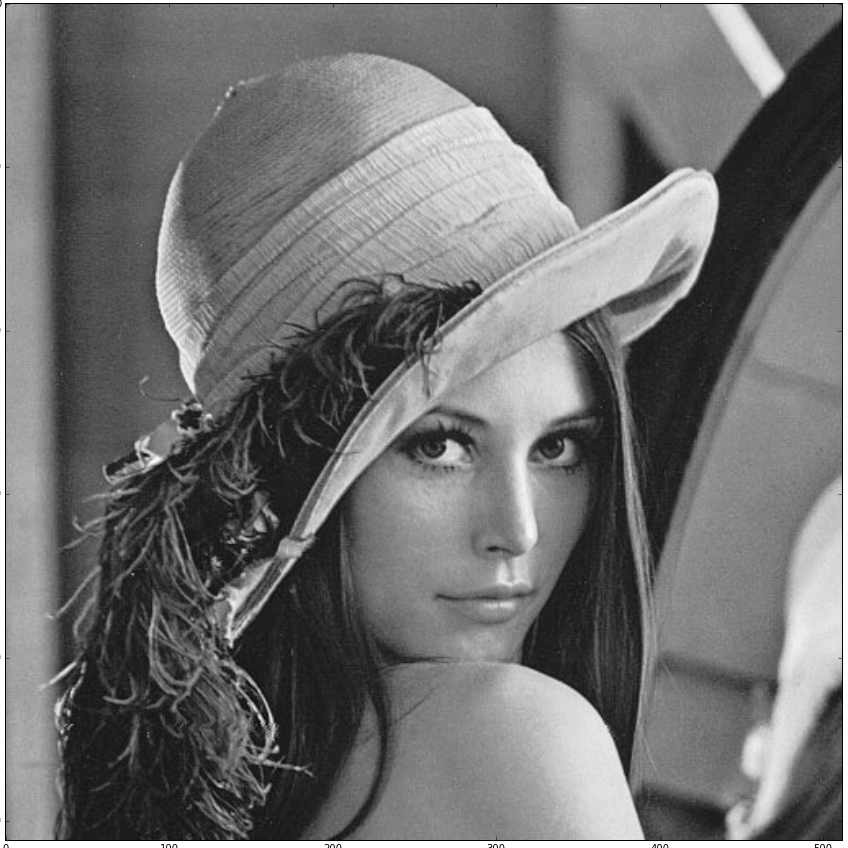
\includegraphics[width=\textwidth]{./Lena-gray}
        \caption{\\Original image}
        \label{pic-original-lena}
    \end{subfigure}
    \begin{subfigure}[t]{0.15\textwidth}
        \centering
        \captionsetup{justification=centering,margin=0.1cm}
        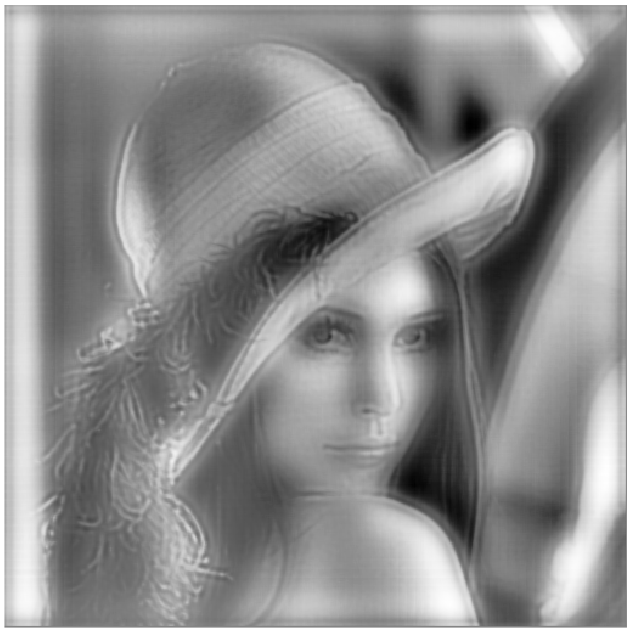
\includegraphics[width=\textwidth]{./final_results-unfiltered}
        \caption{\\100\% raw spikes}
        \label{pic-unfiltered-spikes}
    \end{subfigure}
    %        \hfill
    \begin{subfigure}[t]{0.15\textwidth}
        \centering
        \captionsetup{justification=centering,margin=0.1cm}
        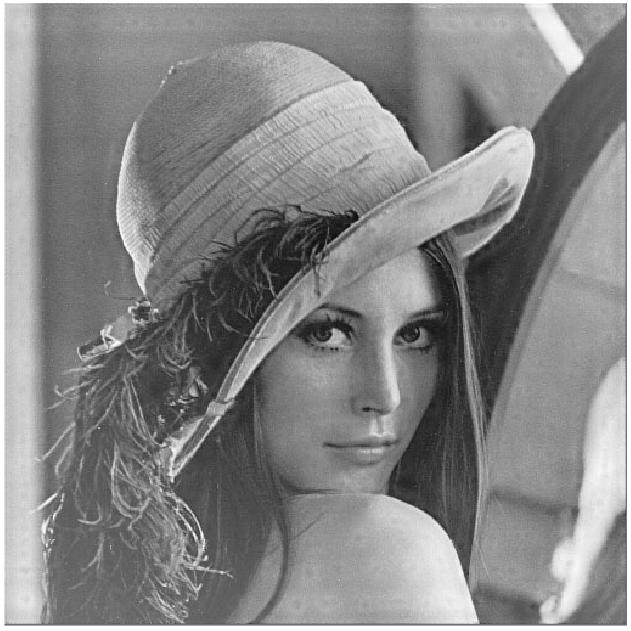
\includegraphics[width=\textwidth]{./final_results-focal-100}
        \caption{\\100\% \emph{corrected} spikes}
        \label{pic-100pc-spikes}
    \end{subfigure}
    \begin{subfigure}[t]{0.15\textwidth}
        \centering
        \captionsetup{justification=centering,margin=0.1cm}
        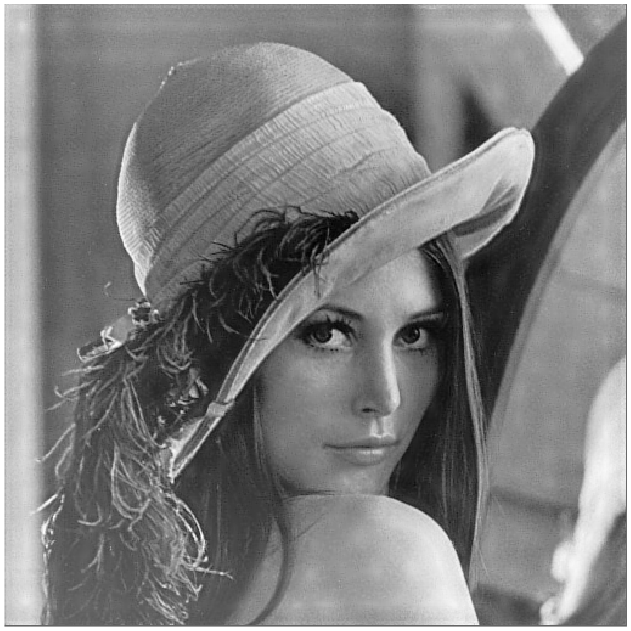
\includegraphics[width=\textwidth]{./final_results-focal-30pc}
        \caption{\\30\% of \emph{corrected} spikes}
        \label{pic-30pc-spikes}
    \end{subfigure}
    \caption{Results of reconstruction procedure}
\end{figure}